\documentclass[aspectratio=169,11pt,t]{beamer}
\usepackage[T1]{fontenc}
\usepackage{mathptmx}
\usepackage[scaled=.92]{helvet}
\usepackage{booktabs,tikz}
\usetikzlibrary{arrows.meta}
\definecolor{gradOrange}{HTML}{F07F3C}
\definecolor{gradPurple}{HTML}{B84FC2}
\definecolor{iiscOrange}{gray}{0.45}
\definecolor{iiscPurple}{gray}{0.1}
\definecolor{accP}{HTML}{5F4B6B}
\definecolor{accA}{HTML}{C58A63}
\setbeamercolor{background canvas}{bg=white!99!black}
\setbeamercolor{structure}{fg=iiscPurple}
\setbeamercolor{itemize item}{fg=iiscOrange}
\setbeamercolor{itemize subitem}{fg=iiscPurple}
\setbeamerfont{frametitle}{series=\bfseries,size=\LARGE}
\setbeamertemplate{navigation symbols}{}
\setbeamertemplate{itemize item}[square]
\setbeamertemplate{frametitle}{\vskip1.1ex{\color{black}\sffamily\bfseries\LARGE\insertframetitle}\par\vskip1.2ex}
\setbeamertemplate{background}{\vbox to\paperheight{\vfill\hbox to\paperwidth{%
  \tikz[baseline=0]\shade[left color=gradOrange,right color=gradPurple] (0,0) rectangle (\paperwidth,.16);}}}
\setbeamertemplate{footline}{\hfill{\color{black!35}\fontsize{7}{8}\selectfont\insertframenumber/\inserttotalframenumber}\hspace*{.85cm}\vskip4.6ex}
\setbeamersize{text margin left=1.6cm,text margin right=1.6cm}
\usepackage{amsmath,amssymb}
\newcommand{\rAgree}{93.8}
\newcommand{\rBattM}{71.1}
\newcommand{\rBattR}{63.5}
\newcommand{\rBothVan}{21.3}
\newcommand{\rBusyHigM}{21.8}
\newcommand{\rBusyHigR}{21.9}
\newcommand{\rBusyLowM}{6.2}
\newcommand{\rBusyLowR}{6.6}
\newcommand{\rBusyMedM}{23.3}
\newcommand{\rBusyMedR}{23.9}
\newcommand{\rComVanHighM}{98.1}
\newcommand{\rComVanHighR}{99.0}
\newcommand{\rComVanM}{103}
\newcommand{\rComVanR}{99}
\newcommand{\rComVanTLM}{100.0}
\newcommand{\rComVanTLR}{100.0}
\newcommand{\rComVanWaitM}{129.2}
\newcommand{\rComVanWaitR}{175.6}
\newcommand{\rCutHi}{0.69}
\newcommand{\rCutLo}{0.17}
\newcommand{\rDirAgree}{13}
\newcommand{\rDirMaxDiff}{0.41}
\newcommand{\rDirTotal}{15}
\newcommand{\rDrivePoorM}{2.69}
\newcommand{\rDrivePoorR}{2.81}
\newcommand{\rDriveRichM}{1.83}
\newcommand{\rDriveRichR}{1.97}
\newcommand{\rFleetM}{43.9}
\newcommand{\rFleetR}{41.6}
\newcommand{\rFullM}{48.1}
\newcommand{\rFullR}{19.4}
\newcommand{\rGapHundred}{1.02}
\newcommand{\rGapMean}{0.85}
\newcommand{\rGapMed}{0.76}
\newcommand{\rGapOpt}{0.92}
\newcommand{\rGunLongM}{7.8}
\newcommand{\rGunLongR}{8.1}
\newcommand{\rGunM}{12.8}
\newcommand{\rGunMaxM}{91.4}
\newcommand{\rGunMaxR}{92.4}
\newcommand{\rGunNeverM}{29.0}
\newcommand{\rGunNeverR}{25.6}
\newcommand{\rGunR}{13.3}
\newcommand{\rGunShortM}{19.4}
\newcommand{\rGunShortR}{20.1}
\newcommand{\rIdleGunsM}{7.0}
\newcommand{\rIdleGunsR}{6.1}
\newcommand{\rLostmBattery}{1}
\newcommand{\rLostmDemandHi}{--}
\newcommand{\rLostmDemandLo}{--}
\newcommand{\rLostmGunsFour}{--}
\newcommand{\rLostmGunsOne}{--}
\newcommand{\rLostmOmegaHi}{2}
\newcommand{\rLostmPersCHi}{2}
\newcommand{\rLostmPowerHi}{--}
\newcommand{\rLostmPowerLo}{--}
\newcommand{\rLostmSeatsFour}{7}
\newcommand{\rLostmTariffHi}{0}
\newcommand{\rLostmTariffLo}{4}
\newcommand{\rLostmTaxiMuHi}{1}
\newcommand{\rLostmTaxiMuLo}{0}
\newcommand{\rLostmVansSeven}{0}
\newcommand{\rLostmVansThree}{33}
\newcommand{\rLostrBattery}{1}
\newcommand{\rLostrDemandHi}{79}
\newcommand{\rLostrDemandLo}{0}
\newcommand{\rLostrGunsFour}{0}
\newcommand{\rLostrGunsOne}{68}
\newcommand{\rLostrOmegaHi}{1}
\newcommand{\rLostrPersCHi}{0}
\newcommand{\rLostrPowerHi}{0}
\newcommand{\rLostrPowerLo}{102}
\newcommand{\rLostrSeatsFour}{6}
\newcommand{\rLostrTariffHi}{1}
\newcommand{\rLostrTariffLo}{1}
\newcommand{\rLostrTaxiMuHi}{1}
\newcommand{\rLostrTaxiMuLo}{0}
\newcommand{\rLostrVansSeven}{0}
\newcommand{\rLostrVansThree}{34}
\newcommand{\rNPairedR}{474}
\newcommand{\rNValidM}{474}
\newcommand{\rNValidR}{500}
\newcommand{\rNewmBattery}{3}
\newcommand{\rNewmDemandHi}{--}
\newcommand{\rNewmDemandLo}{--}
\newcommand{\rNewmGunsFour}{--}
\newcommand{\rNewmGunsOne}{--}
\newcommand{\rNewmOmegaHi}{3}
\newcommand{\rNewmPersCHi}{1}
\newcommand{\rNewmPowerHi}{--}
\newcommand{\rNewmPowerLo}{--}
\newcommand{\rNewmSeatsFour}{4}
\newcommand{\rNewmTariffHi}{3}
\newcommand{\rNewmTariffLo}{1}
\newcommand{\rNewmTaxiMuHi}{2}
\newcommand{\rNewmTaxiMuLo}{1}
\newcommand{\rNewmVansSeven}{13}
\newcommand{\rNewmVansThree}{0}
\newcommand{\rNewrBattery}{1}
\newcommand{\rNewrDemandHi}{0}
\newcommand{\rNewrDemandLo}{39}
\newcommand{\rNewrGunsFour}{9}
\newcommand{\rNewrGunsOne}{0}
\newcommand{\rNewrOmegaHi}{0}
\newcommand{\rNewrPersCHi}{0}
\newcommand{\rNewrPowerHi}{32}
\newcommand{\rNewrPowerLo}{0}
\newcommand{\rNewrSeatsFour}{0}
\newcommand{\rNewrTariffHi}{1}
\newcommand{\rNewrTariffLo}{0}
\newcommand{\rNewrTaxiMuHi}{1}
\newcommand{\rNewrTaxiMuLo}{0}
\newcommand{\rNewrVansSeven}{6}
\newcommand{\rNewrVansThree}{0}
\newcommand{\rQShareComM}{91.7}
\newcommand{\rQShareComR}{94.2}
\newcommand{\rQSharePoorM}{76.0}
\newcommand{\rQSharePoorR}{72.8}
\newcommand{\rQUserComM}{74.2}
\newcommand{\rQUserComR}{71.1}
\newcommand{\rQUserPoorM}{49.2}
\newcommand{\rQUserPoorR}{47.2}
\newcommand{\rQueueComHigM}{7.04}
\newcommand{\rQueueComHigR}{10.49}
\newcommand{\rQueueComLowM}{0.04}
\newcommand{\rQueueComLowR}{0.16}
\newcommand{\rQueueComMedM}{0.33}
\newcommand{\rQueueComMedR}{0.89}
\newcommand{\rQueueHiPoorM}{8.35}
\newcommand{\rQueueHiPoorR}{11.44}
\newcommand{\rQueueHiRichM}{0.16}
\newcommand{\rQueueHiRichR}{0.44}
\newcommand{\rQueueHigM}{5.52}
\newcommand{\rQueueHigR}{7.65}
\newcommand{\rQueueLowM}{0.03}
\newcommand{\rQueueLowR}{0.12}
\newcommand{\rQueueMedM}{0.26}
\newcommand{\rQueueMedR}{0.67}
\newcommand{\rQueuePersHigM}{1.67}
\newcommand{\rQueuePersHigR}{1.45}
\newcommand{\rQueuePersLowM}{0.00}
\newcommand{\rQueuePersLowR}{0.02}
\newcommand{\rQueuePersMedM}{0.06}
\newcommand{\rQueuePersMedR}{0.12}
\newcommand{\rQueuedHigM}{30.3}
\newcommand{\rQueuedHigR}{35.6}
\newcommand{\rQueuedLowM}{0.5}
\newcommand{\rQueuedLowR}{1.2}
\newcommand{\rQueuedMedM}{3.1}
\newcommand{\rQueuedMedR}{5.6}
\newcommand{\rRlBetter}{28}
\newcommand{\rRlEqual}{50}
\newcommand{\rRlOnly}{26}
\newcommand{\rRoadM}{68.4}
\newcommand{\rRoadR}{68.6}
\newcommand{\rSeatsM}{79.0}
\newcommand{\rSeatsR}{69.4}
\newcommand{\rShareHigM}{21.6}
\newcommand{\rShareHigR}{21.6}
\newcommand{\rShareLowM}{46.9}
\newcommand{\rShareLowR}{46.9}
\newcommand{\rShareMedM}{31.5}
\newcommand{\rShareMedR}{31.5}
\newcommand{\rThetaFcsM}{0.43}
\newcommand{\rThetaFcsR}{0.45}
\newcommand{\rThetaVanM}{0.89}
\newcommand{\rThetaVanR}{0.86}
\newcommand{\rTimeM}{139.7}
\newcommand{\rTimeMHundred}{217.1}
\newcommand{\rTimeR}{0.12}
\newcommand{\rTimeRHundred}{0.22}
\newcommand{\rVanChargeM}{35.4}
\newcommand{\rVanChargeR}{31.7}
\newcommand{\rVanComHigM}{3.4}
\newcommand{\rVanComHigR}{3.3}
\newcommand{\rVanComLowM}{0.0}
\newcommand{\rVanComLowR}{0.0}
\newcommand{\rVanComM}{0.7}
\newcommand{\rVanComMedM}{0.0}
\newcommand{\rVanComMedR}{0.0}
\newcommand{\rVanComR}{0.7}
\newcommand{\rVanEnergyM}{20.1}
\newcommand{\rVanEnergyR}{16.9}
\newcommand{\rVanPersBelowFourM}{0.0}
\newcommand{\rVanPersBelowFourR}{0.0}
\newcommand{\rVanPersHigM}{16.6}
\newcommand{\rVanPersHigR}{2.6}
\newcommand{\rVanPersLowM}{23.4}
\newcommand{\rVanPersLowR}{9.4}
\newcommand{\rVanPersM}{19.9}
\newcommand{\rVanPersMedM}{17.1}
\newcommand{\rVanPersMedR}{4.8}
\newcommand{\rVanPersR}{6.4}
\newcommand{\rVanPersSixEightM}{9.8}
\newcommand{\rVanPersSixEightR}{4.1}
\newcommand{\rVanPersTopM}{49.7}
\newcommand{\rVanPersTopR}{10.9}
\newcommand{\rVanWaitM}{38.2}
\newcommand{\rVanWaitR}{41.6}
\newcommand{\rVansLongSeatsM}{89.1}
\newcommand{\rVansLongSeatsR}{78.2}
\newcommand{\rVansM}{1040}
\newcommand{\rVansR}{985}
\newcommand{\rVansShortRoadM}{86.3}
\newcommand{\rVansShortRoadR}{84.3}
\newcommand{\rVansShortSeatsM}{47.2}
\newcommand{\rVansShortSeatsR}{43.0}
\newcommand{\rdVPmBattery}{$-$1.4}
\newcommand{\rdVPmDemandHi}{--}
\newcommand{\rdVPmDemandLo}{--}
\newcommand{\rdVPmGunsFour}{--}
\newcommand{\rdVPmGunsOne}{--}
\newcommand{\rdVPmOmegaHi}{$-$0.3}
\newcommand{\rdVPmPersCHi}{+9.5}
\newcommand{\rdVPmPowerHi}{--}
\newcommand{\rdVPmPowerLo}{--}
\newcommand{\rdVPmSeatsFour}{$-$8.2}
\newcommand{\rdVPmTariffHi}{$-$6.4}
\newcommand{\rdVPmTariffLo}{+11.6}
\newcommand{\rdVPmTaxiMuHi}{$-$0.1}
\newcommand{\rdVPmTaxiMuLo}{$-$0.3}
\newcommand{\rdVPmVansSeven}{+0.6}
\newcommand{\rdVPmVansThree}{$-$2.0}
\newcommand{\rdVPrBattery}{+1.4}
\newcommand{\rdVPrDemandHi}{$-$0.8}
\newcommand{\rdVPrDemandLo}{$-$0.6}
\newcommand{\rdVPrGunsFour}{$-$1.4}
\newcommand{\rdVPrGunsOne}{+10.6}
\newcommand{\rdVPrOmegaHi}{+0.3}
\newcommand{\rdVPrPersCHi}{+5.0}
\newcommand{\rdVPrPowerHi}{$-$6.7}
\newcommand{\rdVPrPowerLo}{+52.4}
\newcommand{\rdVPrSeatsFour}{+0.5}
\newcommand{\rdVPrTariffHi}{$-$5.6}
\newcommand{\rdVPrTariffLo}{+4.6}
\newcommand{\rdVPrTaxiMuHi}{+1.0}
\newcommand{\rdVPrTaxiMuLo}{+0.4}
\newcommand{\rdVPrVansSeven}{+0.3}
\newcommand{\rdVPrVansThree}{$-$0.5}
\newcommand{\rdZmBattery}{$-$0.01}
\newcommand{\rdZmDemandHi}{--}
\newcommand{\rdZmDemandLo}{--}
\newcommand{\rdZmGunsFour}{--}
\newcommand{\rdZmGunsOne}{--}
\newcommand{\rdZmOmegaHi}{+2.66}
\newcommand{\rdZmPersCHi}{+2.08}
\newcommand{\rdZmPowerHi}{--}
\newcommand{\rdZmPowerLo}{--}
\newcommand{\rdZmSeatsFour}{+1.08}
\newcommand{\rdZmTariffHi}{+3.91}
\newcommand{\rdZmTariffLo}{$-$4.19}
\newcommand{\rdZmTaxiMuHi}{+6.43}
\newcommand{\rdZmTaxiMuLo}{$-$6.38}
\newcommand{\rdZmVansSeven}{+0.02}
\newcommand{\rdZmVansThree}{$-$0.04}
\newcommand{\rdZrBattery}{$-$0.07}
\newcommand{\rdZrDemandHi}{+22.19}
\newcommand{\rdZrDemandLo}{$-$21.82}
\newcommand{\rdZrGunsFour}{$-$2.21}
\newcommand{\rdZrGunsOne}{+4.76}
\newcommand{\rdZrOmegaHi}{+2.75}
\newcommand{\rdZrPersCHi}{+2.38}
\newcommand{\rdZrPowerHi}{$-$12.30}
\newcommand{\rdZrPowerLo}{+20.13}
\newcommand{\rdZrSeatsFour}{+0.88}
\newcommand{\rdZrTariffHi}{+3.73}
\newcommand{\rdZrTariffLo}{$-$3.78}
\newcommand{\rdZrTaxiMuHi}{+6.33}
\newcommand{\rdZrTaxiMuLo}{$-$6.25}
\newcommand{\rdZrVansSeven}{+0.00}
\newcommand{\rdZrVansThree}{+0.09}

\newcommand{\slidefoot}[1]{\par\vfill{\tiny\color{black!55}#1}\par\vspace{.4ex}}

\begin{document}

% =================================================================== 1 MILP infrastructure
\begin{frame}{Results (MILP): infrastructure use}
\begin{columns}[T]
\column{.58\textwidth}
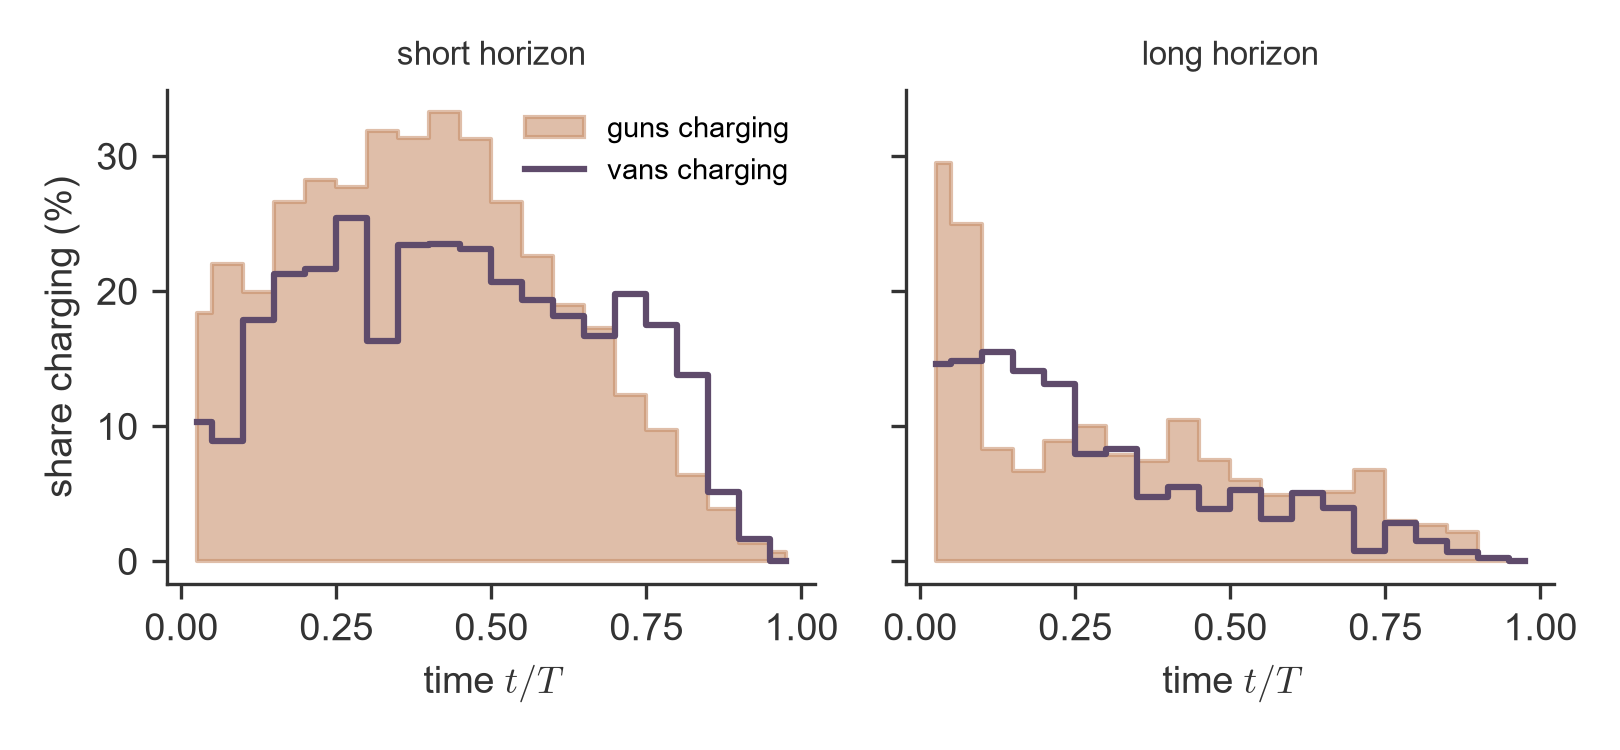
\includegraphics[width=\textwidth]{figures/res_infra_M.png}

\scriptsize\setlength{\tabcolsep}{3pt}
\begin{tabular}{lr@{\hspace{10pt}}lr}
\toprule
guns busy over $[0,T]$ & \rGunM\% & vans sent (of 5) & \rFleetM\%\\
short / long horizon & \rGunShortM{} / \rGunLongM\% & seats used & \rSeatsM\%\\
idle guns (of 24) & \rIdleGunsM & vans full & \rFullM\%\\
guns never used & \rGunNeverM\% & battery used & \rBattM\%\\
\bottomrule
\end{tabular}
\column{.39\textwidth}
\small
\begin{itemize}
  \item Guns idle most of the time; demand comes in bursts.
  \item Long horizons: busiest at the start, then nearly idle.
  \item Vans: \rRoadM\% of $T$ on the road; \rVanChargeM\% of it charging, \rVanWaitM\% waiting.
  \item Short horizons: vans run out of \textbf{time}; long: of \textbf{seats} (\rVansLongSeatsM\%).
\end{itemize}
\end{columns}
\slidefoot{MILP on the \rNPairedR{} instances both methods solve; means over plans and dispatched vans.}
\end{frame}

% =================================================================== 2 MILP income
\begin{frame}{Results (MILP): income and segment}
\begin{columns}[T]
\column{.58\textwidth}
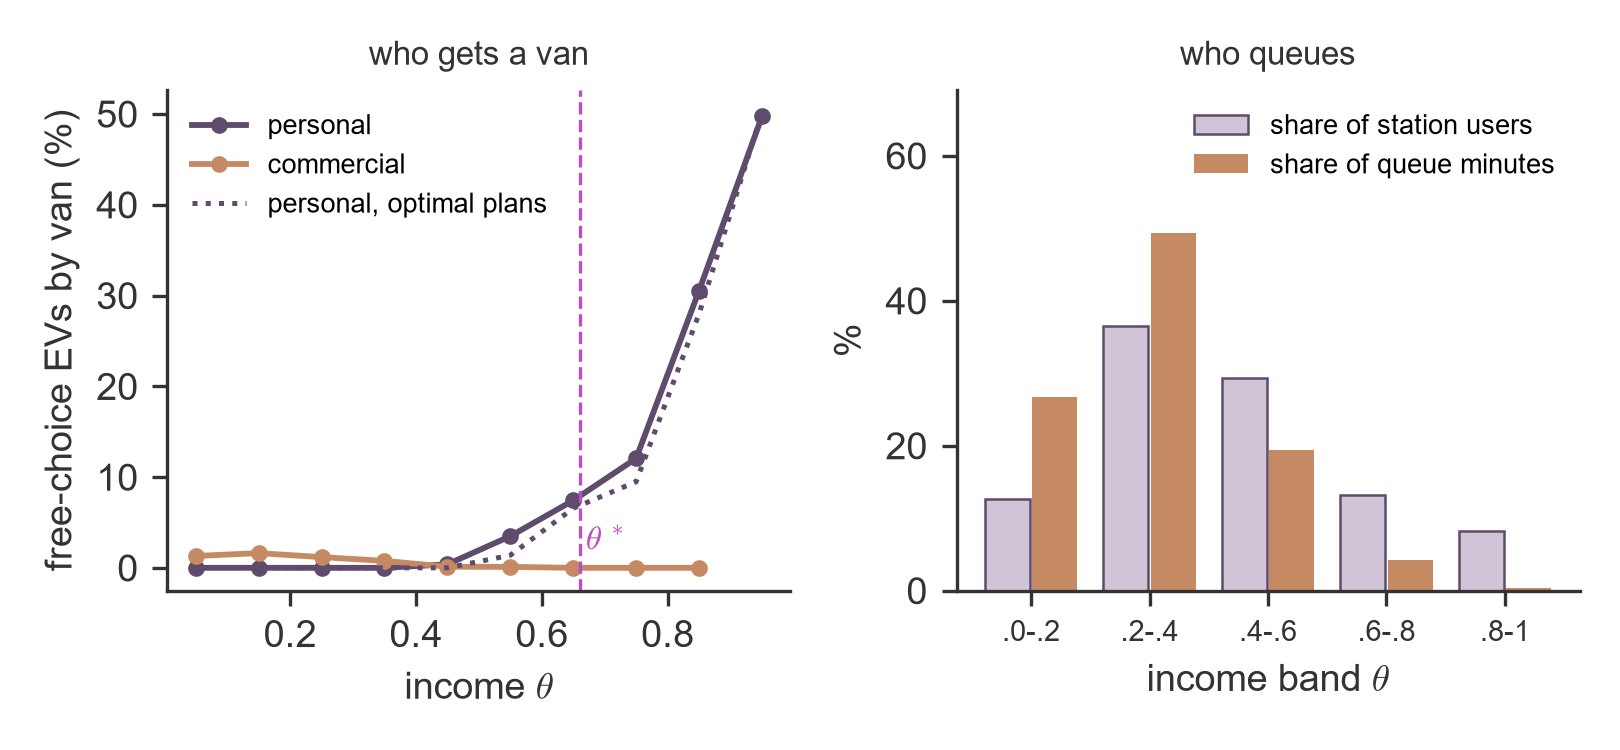
\includegraphics[width=\textwidth]{figures/res_income_M.png}
\column{.39\textwidth}
\small
\begin{itemize}
  \item Personal by van: \rVanPersM\%; 0\% below $\theta=0.4$, \rVanPersTopM\% above 0.9.
  \item The step sits at theory's $\theta^*=0.66$.
  \item Taxis by van: \rVanComM\%, all in unfinished plans.
  \item Taxis: \rQUserComM\% of station users, \rQShareComM\% of queue time.
  \item $\theta<0.4$: \rQUserPoorM\% of users, \rQSharePoorM\% of queue time.
\end{itemize}
\end{columns}
\slidefoot{Free-choice EVs (a station in range). Dotted: proven-optimal plans only.}
\end{frame}

% =================================================================== 3 MILP demand pressure
\begin{frame}{Results (MILP): demand pressure}
\begin{columns}[T]
\column{.58\textwidth}
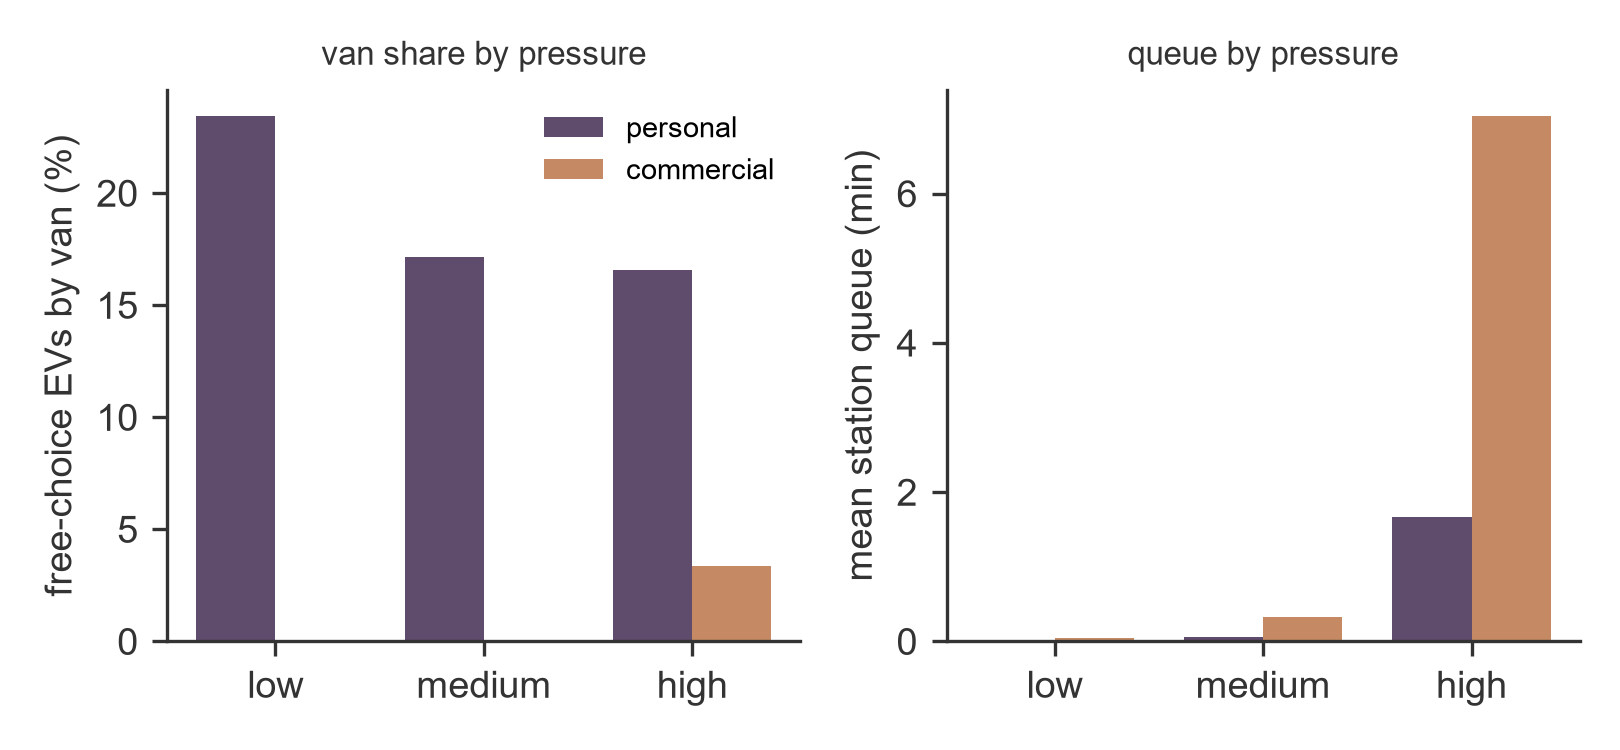
\includegraphics[width=\textwidth]{figures/res_pressure_M.png}
\column{.39\textwidth}
\small
\begin{itemize}
  \item Queues only at high pressure: \rQueueLowM{} / \rQueueMedM{} / \rQueueHigM{} min.
  \item Users queueing: \rQueuedLowM\% $\to$ \rQueuedHigM\%.
  \item Taxis use vans only at high pressure (\rVanComHigM\%).
  \item Personal vans fall: \rVanPersLowM\% $\to$ \rVanPersHigM\%.
  \item High pressure: \rQueueHiPoorM{} min ($\theta<0.4$) vs \rQueueHiRichM{} ($\theta\ge0.8$).
\end{itemize}
\end{columns}
\slidefoot{Pressure of EV $i$ = requests in the last average charging time / 29 chargers; low $\le$ \rCutLo, high $>$ \rCutHi{} (terciles, all 560 instances).}
\end{frame}

% =================================================================== 4 RL infrastructure
\begin{frame}{Results (RL): infrastructure use}
\begin{columns}[T]
\column{.58\textwidth}
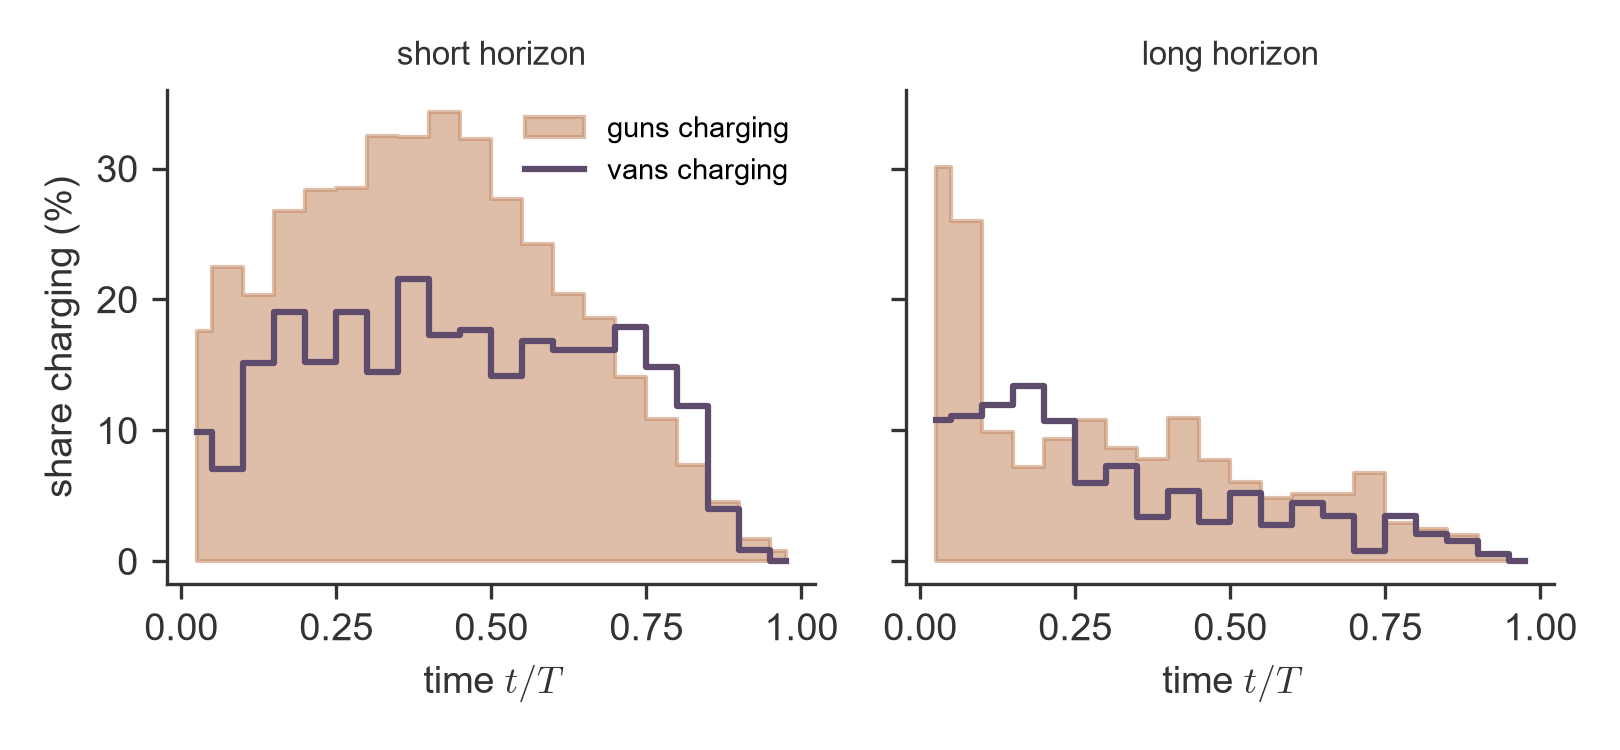
\includegraphics[width=\textwidth]{figures/res_infra_R.png}

\scriptsize\setlength{\tabcolsep}{3pt}
\begin{tabular}{lr@{\hspace{10pt}}lr}
\toprule
guns busy over $[0,T]$ & \rGunR\% & vans sent (of 5) & \rFleetR\%\\
short / long horizon & \rGunShortR{} / \rGunLongR\% & seats used & \rSeatsR\%\\
idle guns (of 24) & \rIdleGunsR & vans full & \rFullR\%\\
guns never used & \rGunNeverR\% & battery used & \rBattR\%\\
\bottomrule
\end{tabular}
\column{.39\textwidth}
\small
\begin{itemize}
  \item Same time profile as the MILP.
  \item Leans on stations: guns busier, fewer idle.
  \item Emptier vans: \rFullR\% full (MILP \rFullM\%).
  \item Van road time: \rVanChargeR\% charging, \rVanWaitR\% waiting.
  \item Energy by van: \rVanEnergyR\% (MILP \rVanEnergyM\%).
\end{itemize}
\end{columns}
\slidefoot{RL on the same \rNPairedR{} instances; means over plans and dispatched vans.}
\end{frame}

% =================================================================== 5 RL income
\begin{frame}{Results (RL): income and segment}
\begin{columns}[T]
\column{.58\textwidth}
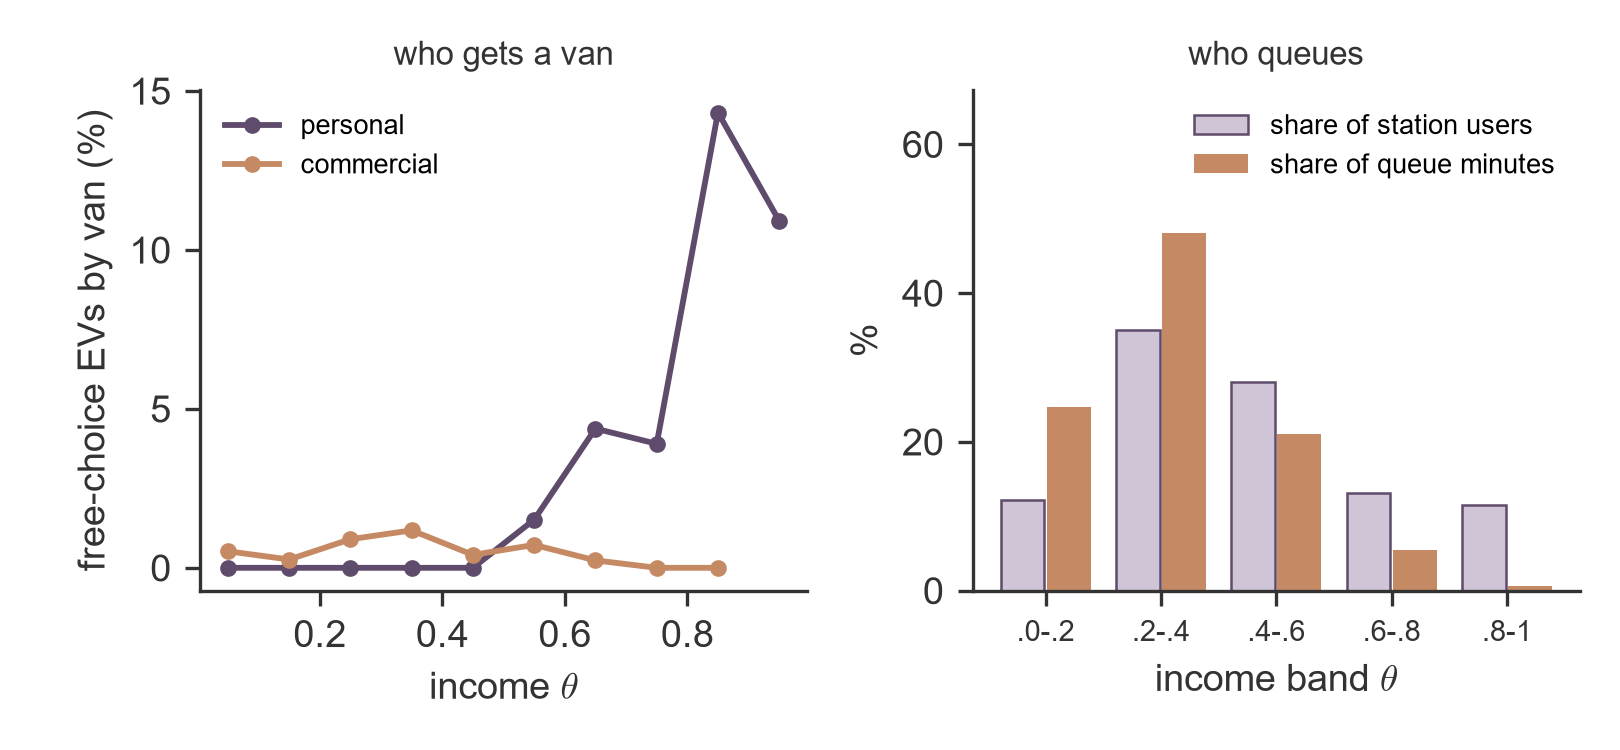
\includegraphics[width=\textwidth]{figures/res_income_R.png}
\column{.39\textwidth}
\small
\begin{itemize}
  \item Same order as the MILP, weaker: personal by van \rVanPersR\%, \rVanPersTopR\% above $\theta=0.9$.
  \item Van users rich ($\bar\theta=$ \rThetaVanR), station users not (\rThetaFcsR).
  \item Taxis by van: \rVanComR\%.
  \item Taxis do \rQShareComR\% of the queueing.
  \item $\theta<0.4$: \rQSharePoorR\% of queue time.
\end{itemize}
\end{columns}
\slidefoot{Free-choice EVs of the \rNPairedR{} paired instances.}
\end{frame}

% =================================================================== 6 RL demand pressure
\begin{frame}{Results (RL): demand pressure}
\begin{columns}[T]
\column{.58\textwidth}
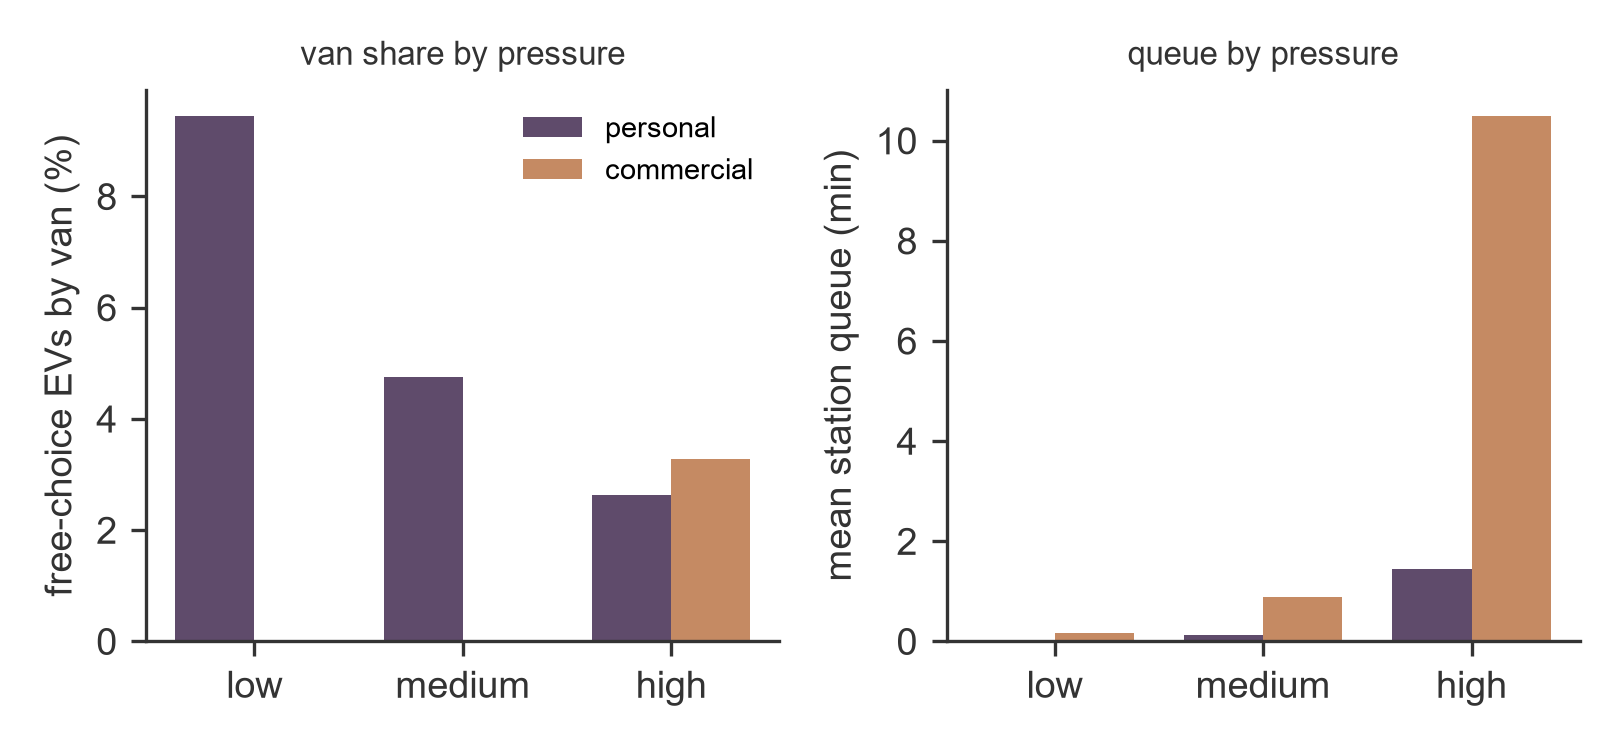
\includegraphics[width=\textwidth]{figures/res_pressure_R.png}
\column{.39\textwidth}
\small
\begin{itemize}
  \item Queues: \rQueueLowR{} / \rQueueMedR{} / \rQueueHigR{} min; longer than the MILP at high pressure.
  \item Users queueing at high pressure: \rQueuedHigR\%.
  \item Taxis use vans only at high pressure (\rVanComHigR\%).
  \item Personal vans fall faster: \rVanPersLowR\% $\to$ \rVanPersHigR\%.
  \item High pressure: \rQueueHiPoorR{} min ($\theta<0.4$) vs \rQueueHiRichR{} ($\theta\ge0.8$).
\end{itemize}
\end{columns}
\end{frame}

% =================================================================== 7 combined
\begin{frame}{Results: MILP and RL combined}
\begin{columns}[T]
\column{.58\textwidth}
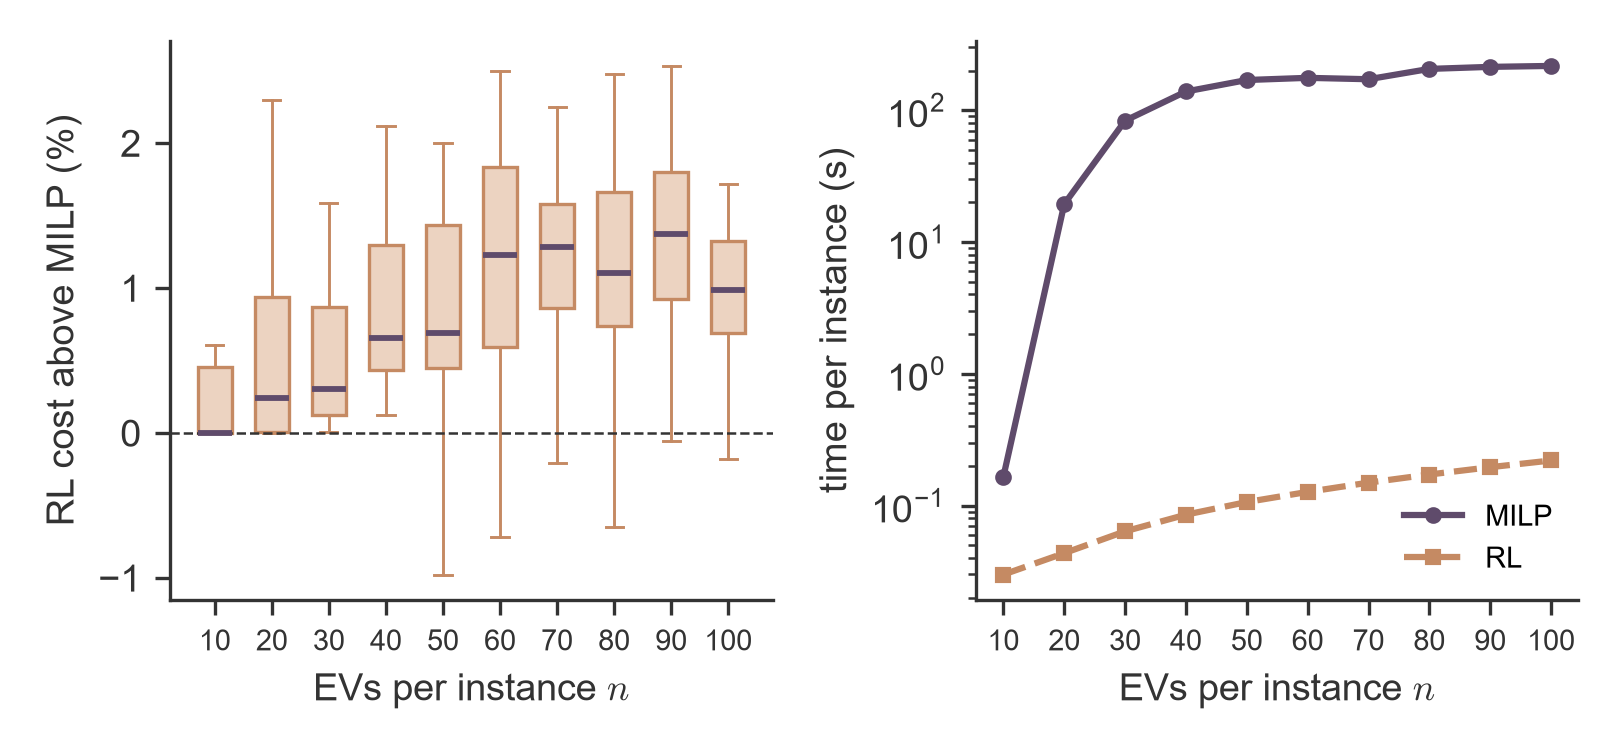
\includegraphics[width=\textwidth]{figures/res_combined.png}

\scriptsize\setlength{\tabcolsep}{3pt}
\begin{tabular}{lrr}
\toprule
 & MILP & RL\\
\midrule
valid plans (of 560) & \rNValidM & \rNValidR\\
time per instance, $n=100$ & \rTimeMHundred\,s & \rTimeRHundred\,s\\
personal / taxi by van & \rVanPersM{} / \rVanComM\% & \rVanPersR{} / \rVanComR\%\\
guns busy / vans full & \rGunM{} / \rFullM\% & \rGunR{} / \rFullR\%\\
\bottomrule
\end{tabular}
\column{.39\textwidth}
\small
\begin{itemize}
  \item RL: +\rGapMean\% cost (median \rGapMed\%).
  \item Equal in \rRlEqual, better than the MILP's time-limit plan in \rRlBetter.
  \item RL plans \rRlOnly{} instances the MILP cannot.
  \item Same charger type for \rAgree\% of EVs.
\end{itemize}
\end{columns}
\end{frame}

% =================================================================== 8 experiments
\begin{frame}{Additional experiments and sensitivities}
\begin{columns}[T]
\column{.47\textwidth}
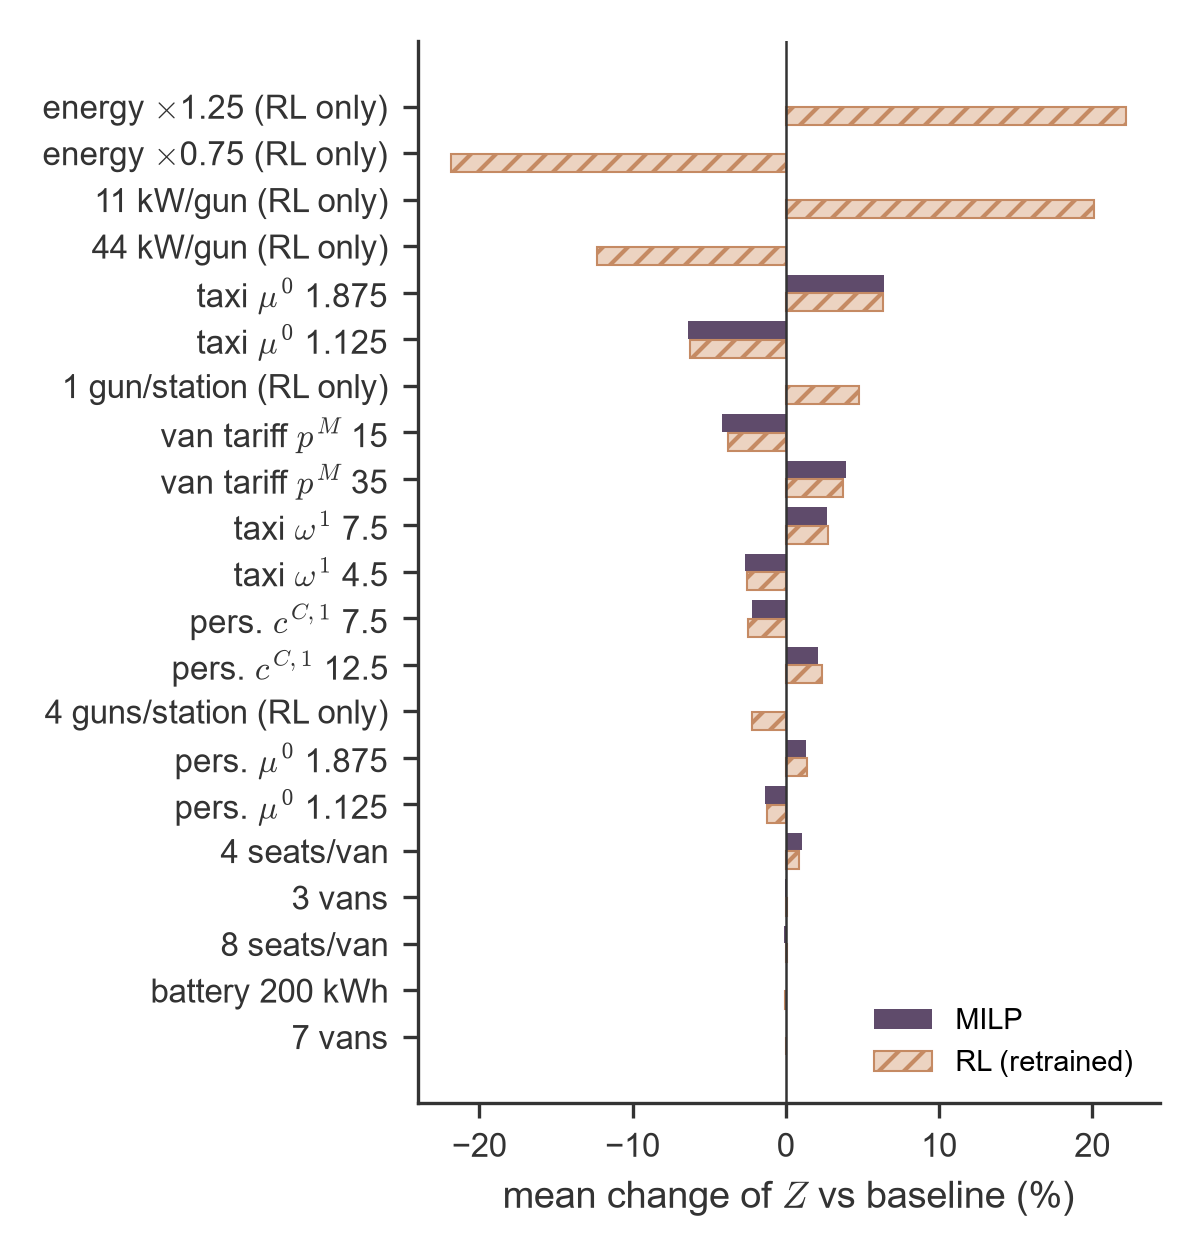
\includegraphics[height=5.3cm]{figures/res_experiments.png}
\column{.5\textwidth}
\scriptsize
\begin{itemize}
  \item \textbf{Taxi money sensitivity} moves $Z$ most: \rdZmTaxiMuLo\% / \rdZmTaxiMuHi\%.
  \item \textbf{Van tariff} 15 / 35: $Z$ \rdZmTariffLo\% / \rdZmTariffHi\%; personal vans \rdVPmTariffLo{} / \rdVPmTariffHi{} pts.
  \item \textbf{Fleet}: 3 vans lose \rLostmVansThree{} instances, 7 vans gain \rNewmVansSeven; cost flat. \textbf{Battery} 200\,kWh: \rdZmBattery\%.
  \item \textbf{Station power}\textsuperscript{RL}: 11\,kW $Z$ \rdZrPowerLo\% (\rLostrPowerLo{} lost); 44\,kW \rdZrPowerHi\%.
  \item \textbf{Guns per station}\textsuperscript{RL}: 1 gives \rdZrGunsOne\%, 4 gives \rdZrGunsFour\%.
  \item \textbf{Energy per EV} $\pm25\%$\textsuperscript{RL}: $Z$ \rdZrDemandLo\% / \rdZrDemandHi\%.
  \item RL follows the MILP's direction in \rDirAgree{} of \rDirTotal{} shared variants.
\end{itemize}
\end{columns}
\slidefoot{One factor at a time; mean change of $Z$ on instances valid in both runs. RL: retrained model. \textsuperscript{RL} RL only (no MILP run).}
\end{frame}

\end{document}
